\subsection{Rétropropagation}

\begin{frame}{La descente de gradient}
    \begin{block}{Descente de gradient}
        Algorithme permettant de converger vers un minimum local d'une fonction. \\
        Elle est utilisée pour trouver le minimum d'une fonction évaluant l'erreur entre la valeur de sortie du réseau de neurones et celle attendue: \\
        \begin{center}
            $f : s \mapsto (s - s_{attendue})^2$\\
        \end{center}
        - $s$ la sortie donnée par le réseau de neurones \\
        - $s_{attendue}$ la sortie cible. \\

    \end{block}
    \begin{exampleblock}{Objectif}
        Trouver les paramètres pour annuler la fonction d'erreur revient à résoudre le problème qu'elle évalue.
    \end{exampleblock}
\end{frame}


\begin{frame}{Un exemple d'un perceptron seul}
    \begin{figure}
        \centering
        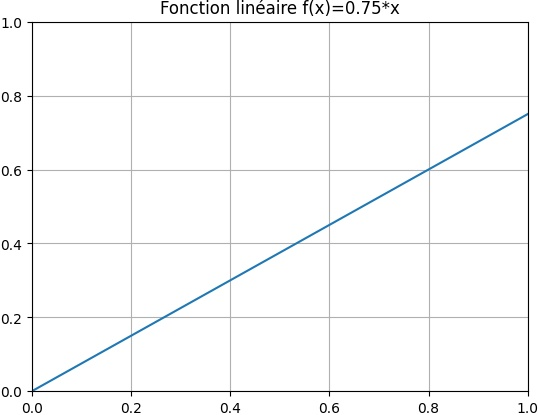
\includegraphics[height=0.5\textheight]{9-fonction_lineaire}
    \end{figure}
    \begin{figure}
        \centering
        
\includegraphics[height=0.2\textheight]{6-Perceptron.png}
        \caption{Schéma d'un perceptron à une entrée}
    \end{figure}
\end{frame}


\begin{frame}{La descente de gradient}
    \begin{block}{Algorithme du gradient}
        $f$ une fonction différentiable de $\mathbb{R} \to \mathbb{R}$. \\
        Soit $x_0$ une valeur initiale aléatoire, $t$ le taux d'apprentissage. \\
        Supposons $x_0, \ldots, x_k$ construits. \\
        • Si $\norme{\nabla f(x_k)} \leq \varepsilon$, on s'arrête. \\
        • Sinon on pose $x_{k+1} = x_k - t \nabla f(x_k)$ \\
    \end{block}
    \begin{figure}
        \centering
        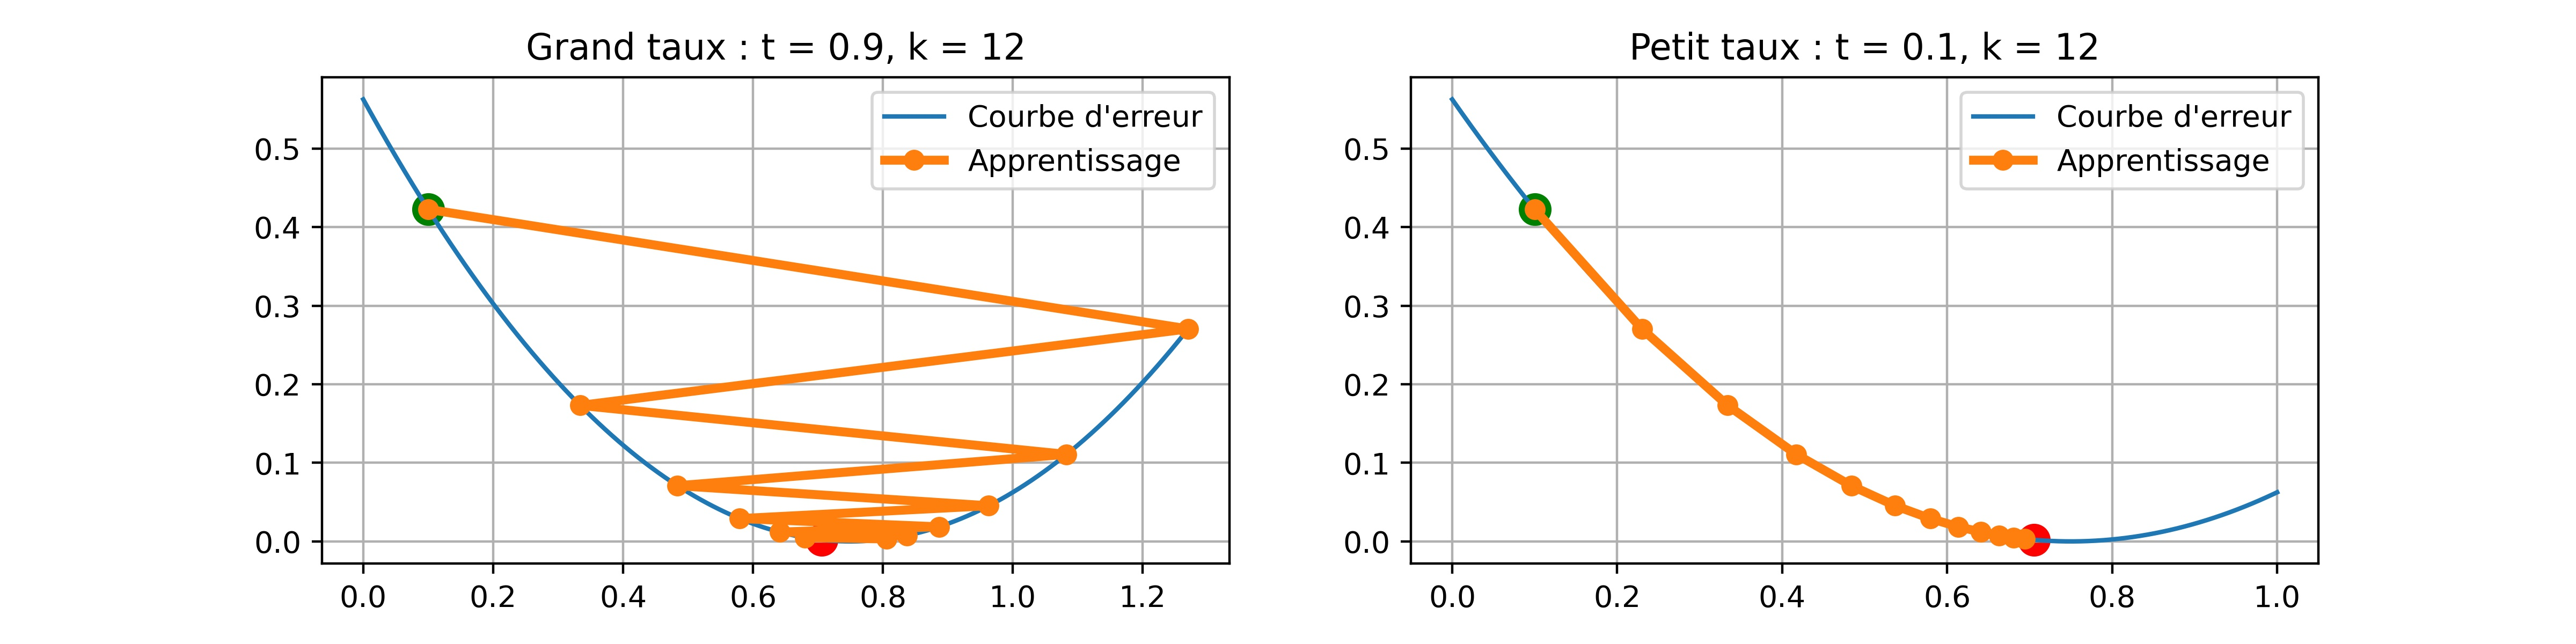
\includegraphics[height=85px]{1-DescenteGradient.jpg}
        \caption{Descente de Gradient pour $f(x) = (x-0.75)^2$; $x_0=0.1$ et $\varepsilon = 0.1$}
    \end{figure}
\end{frame}


